% =====================================================================
% Devoir global de la Journée 1 — Architecture Micro-services
% Compte rendu (Sections 1 à 3). La Section 4 (Lien Git) est exclue.
% Compilation : pdflatex Devoir_J1_compte_rendu.tex   (deux passes)
% =====================================================================
\documentclass[11pt,a4paper]{article}

\usepackage[utf8]{inputenc}
\usepackage[T1]{fontenc}
\usepackage[french]{babel}
\usepackage{mathptmx}            % Times New Roman (texte + maths)
\usepackage[scaled=0.85]{helvet} % sans-serif assorti
\usepackage{courier}             % mono pour le code
\usepackage[margin=2cm]{geometry}
\usepackage{booktabs}
\usepackage{tabularx}
\usepackage{ragged2e}
\usepackage{enumitem}
\usepackage{titlesec}
\usepackage{xcolor}
\usepackage{listings}
\usepackage{graphicx}
\usepackage{float}
\usepackage{caption}
\usepackage{fancyhdr}
\usepackage{lastpage}

\captionsetup{font=small,labelfont=bf,skip=4pt}
\graphicspath{{catalog-service/}{./}}  % trouve swagger-ui.png dans les 2 cas

% ---------- Couleurs sobres (noir & blanc) ----------
\definecolor{gristexte}{gray}{0.35}
\definecolor{codebg}{gray}{0.96}

% ---------- En-tête / pied de page ----------
\pagestyle{fancy}
\fancyhf{}
\fancyfoot[C]{\small\itshape\color{gristexte}Page \thepage}
\renewcommand{\headrulewidth}{0.4pt}
\renewcommand{\footrulewidth}{0pt}

% ---------- Style des titres ----------
\titleformat{\section}{\normalfont\Large\bfseries}{\thesection.}{0.5em}{}[\titlerule]
\titleformat{\subsection}{\normalfont\large\bfseries}{}{0em}{}
\titlespacing*{\section}{0pt}{14pt}{8pt}
\titlespacing*{\subsection}{0pt}{10pt}{4pt}

% ---------- Listes plus compactes ----------
\setlist[itemize]{leftmargin=1.4em,itemsep=2pt,topsep=3pt}

% ---------- Bloc de code ----------
\lstset{
  basicstyle=\ttfamily\small,
  backgroundcolor=\color{codebg},
  frame=none,
  framexleftmargin=4pt,
  xleftmargin=4pt,
  breaklines=true,
  showstringspaces=false,
  columns=fullflexible,
}

% Colonne X justifiée pour tabularx
\newcolumntype{Y}{>{\RaggedRight\arraybackslash}X}

\setlength{\parindent}{0pt}
\setlength{\parskip}{4pt}

\begin{document}

% =====================================================================
% TITRE
% =====================================================================
\thispagestyle{empty}
\begin{center}
  {\LARGE\bfseries Journée 1}\\[4pt]
  {\large\bfseries Architecture Micro-services}\\[6pt]
\end{center}

\vspace{4pt}
\hrule
\vspace{8pt}

Nom / Prénom : DANILO Elouan

\vspace{6pt}

% =====================================================================
% SECTION 1
% =====================================================================
\section{Découpage en services}

Le système retenu est une plateforme de livraison de repas à domicile. Le \textbf{domaine} consiste à mettre en relation trois acteurs (clients, restaurants et livreurs) pour commander un repas, le payer, le faire préparer puis le livrer. Conformément à la règle d'or de la S2, on découpe par \textbf{capacité métier} (ce que le métier fait), jamais par couche technique.

\subsection{Proposition de découpage en 6 services}

\begin{tabularx}{\textwidth}{@{}p{3.2cm}Y p{3.6cm}@{}}
\toprule
\textbf{Service} & \textbf{Capacité métier} & \textbf{Données possédées} \\
\midrule
1. Comptes \& Identité & Inscrire, authentifier et gérer les profils (clients, restaurateurs, livreurs) et les droits d'accès. & Utilisateurs, rôles, adresses, jetons. \\[4pt]
2. Restaurants \& Menus & Présenter l'offre : fiches restaurants, menus, plats, prix, disponibilités et horaires d'ouverture. & Restaurants, menus, plats, catégories. \\[4pt]
3. Commandes & Gérer le cycle de vie d'une commande : panier, validation, suivi des états (créée $\rightarrow$ confirmée $\rightarrow$ préparée $\rightarrow$ livrée). & Commandes, lignes de commande, états. \\[4pt]
4. Paiement & Encaisser, autoriser et rembourser les transactions. Isolé par criticité (audit, sécurité, conformité PCI-DSS). & Transactions, remboursements (réfs). \\[4pt]
5. Livraison & Affecter un livreur, suivre la position GPS, estimer le temps d'arrivée (ETA) et clôturer la course. & Courses, affectations, positions, ETA. \\[4pt]
6. Notifications & Informer chaque acteur en temps réel : push, SMS, email transactionnels (commande confirmée, livreur en route\ldots). & Modèles de messages, journaux d'envoi. \\
\bottomrule
\end{tabularx}

\subsection{Bounded contexts (DDD)}

Chaque service correspond à un \emph{bounded context}, c'est-à-dire une frontière à l'intérieur de laquelle un mot a \textbf{un} sens précis. L'exemple le plus parlant ici est le mot «~Commande~», qui n'a pas le même modèle selon le contexte :

\begin{itemize}
  \item Dans le contexte \textbf{Commandes} (vente), une commande regroupe les plats choisis, le prix, le client et le mode de paiement. États : panier $\rightarrow$ confirmée $\rightarrow$ payée.
  \item Dans le contexte \textbf{Livraison} (logistique), une «~commande~» est une course avec une adresse, une position de livreur, un ETA et un numéro de suivi. États : affectée $\rightarrow$ récupérée $\rightarrow$ livrée.
  \item \textbf{Même mot, deux modèles distincts.} Le DDD valide d'avoir deux bounded contexts. Chaque équipe parle son \emph{ubiquitous language} (ex. «~course~» côté Livraison).
\end{itemize}

D'autres frontières sont nettes. Un «~Restaurant~» côté Restaurants \& Menus (offre, plats) n'est pas le même objet que côté Paiement (un bénéficiaire de versement). Le mot «~Client~» appartient au contexte Comptes \& Identité. Les autres services n'en gardent qu'une référence (l'identifiant).

\subsection{Anti-patterns évités (contrôle S2)}

\begin{itemize}
  \item \textbf{Pas de découpage par couche technique.} Aucun «~service UI~» ni «~service base de données~». Chaque service est une tranche métier verticale.
  \item \textbf{Pas de shared database.} Chaque service possède sa propre base. Les autres passent par l'API, jamais par la table directement.
  \item \textbf{Pas de distributed monolith ni de chatty service.} La confirmation d'une commande n'appelle pas 6 services en synchrone. Le service Commandes publie un événement «~CommandeConfirmée~» que Livraison et Notifications consomment (cohérence à terme, \emph{eventual consistency}).
  \item \textbf{Pas de god service.} Aucun service central ne pilote tous les autres, pas de hub unique.
  \item \textbf{Pas d'entity service.} On a un service «~Commandes~» (capacité), pas un service par table SQL.
  \item \textbf{Paiement isolé par criticité}, un choix volontaire pour la sécurité et l'audit.
\end{itemize}

% =====================================================================
% SECTION 2
% =====================================================================
\newpage
\section{Conception de l'API REST}

Le service retenu est le service \textbf{Commandes}, le cœur transactionnel de la plateforme. L'API suit le style REST (ressources au pluriel, verbes HTTP, codes de statut explicites) et est versionnée par URI (\texttt{/api/v1/}).

\subsection{Endpoints REST (URI + verbe + code de retour)}

\begin{tabularx}{\textwidth}{@{}p{1.6cm} p{5.2cm} Y p{1.8cm}@{}}
\toprule
\textbf{Verbe} & \textbf{URI} & \textbf{Action} & \textbf{Code} \\
\midrule
GET   & \texttt{/api/v1/orders/} & Liste paginée des commandes (filtrable). & 200 \\[3pt]
POST  & \texttt{/api/v1/orders/} & Créer une commande. & 201 \\[3pt]
GET   & \texttt{/api/v1/orders/\{id\}/} & Détail d'une commande. & 200 / 404 \\[3pt]
PATCH & \texttt{/api/v1/orders/\{id\}/} & Modifier partiellement (ex. adresse). & 200 \\[3pt]
GET   & \texttt{/api/v1/orders/\{id\}/items/} & Lignes (plats) de la commande. & 200 \\[3pt]
POST  & \texttt{/api/v1/orders/\{id\}/cancellation/} & Annuler en créant une ressource d'annulation plutôt qu'un verbe \texttt{/cancelOrder}. & 201 / 409 \\[3pt]
GET   & \texttt{/api/v1/orders/\{id\}/tracking/} & État de suivi (délégué à Livraison). & 200 \\
\bottomrule
\end{tabularx}

\vspace{4pt}
Par choix de modélisation, il n'y a pas de DELETE sur une commande. Une commande payée est un fait comptable. On ne la supprime pas, on l'\textbf{annule} (changement d'état via la ressource \texttt{cancellation}). On pense ressources et états, pas actions.

\subsection{Exemple de payload JSON (création, POST /api/v1/orders/)}

\begin{lstlisting}
{
  "customer_id": 42,
  "restaurant_id": 7,
  "delivery_address": "12 rue des Lilas, 75011 Paris",
  "items": [
    { "dish_id": 101, "quantity": 2 },
    { "dish_id": 205, "quantity": 1 }
  ],
  "payment_method": "card"
}
\end{lstlisting}

La réponse \texttt{201 Created} contient la commande créée avec son \texttt{id}, son état initial («~created~»), le total calculé côté serveur (jamais envoyé par le client) et les horodatages \texttt{created\_at} / \texttt{updated\_at}.

\subsection{Pagination, filtrage, tri, versioning}

\begin{itemize}
  \item Le \textbf{versioning} se fait par URI (\texttt{/api/v1/...}). C'est la stratégie la plus lisible et debuggable. L'ancienne version est maintenue 6 à 12 mois en cas de v2.
  \item La \textbf{pagination} utilise \texttt{PageNumberPagination} (\texttt{?page=2\&page\_size=20}) avec la réponse standard \texttt{\{ count, next, previous, results \}}. Pour de gros volumes (historique), on basculerait sur une pagination \emph{cursor-based} (performance constante).
  \item \textbf{Filtrage} par paramètres : \texttt{?status=confirmed}, \texttt{?restaurant=7}, \texttt{?customer=42}.
  \item Le \textbf{tri} se fait avec \texttt{?ordering=-created\_at} (le préfixe \texttt{-} signifie décroissant).
  \item Les \textbf{erreurs structurées} suivent le format RFC 7807 (\texttt{application/problem+json}) avec \texttt{title}, \texttt{detail} et le détail des champs invalides. Jamais de stack trace en production.
\end{itemize}

En cas d'erreur de validation, l'API renvoie par exemple un \texttt{422} avec un corps \texttt{application/problem+json} indiquant que le champ «~items~» ne peut pas être vide, avec un code de statut 4xx (et non 200).

% =====================================================================
% SECTION 3
% =====================================================================
\newpage
\section{Retour sur le TP (service Catalogue)}

Le TP de la S4 a consisté à coder le \textbf{premier} micro-service de FlexShop, le service Catalogue, une API REST CRUD sur la ressource \texttt{Product}, avec Django + Django REST Framework, drf-spectacular (OpenAPI) et django-filter.

\subsection{Documentation OpenAPI : Swagger UI fonctionnel}

La documentation interactive est générée automatiquement par drf-spectacular et servie sur \texttt{/api/docs/}. Elle expose les 7 opérations (CRUD complet + endpoint bonus \texttt{low-stock}) et les schémas (\texttt{Product}, \texttt{PaginatedProductList}, \texttt{PatchedProduct}).

\begin{figure}[H]
  \centering
  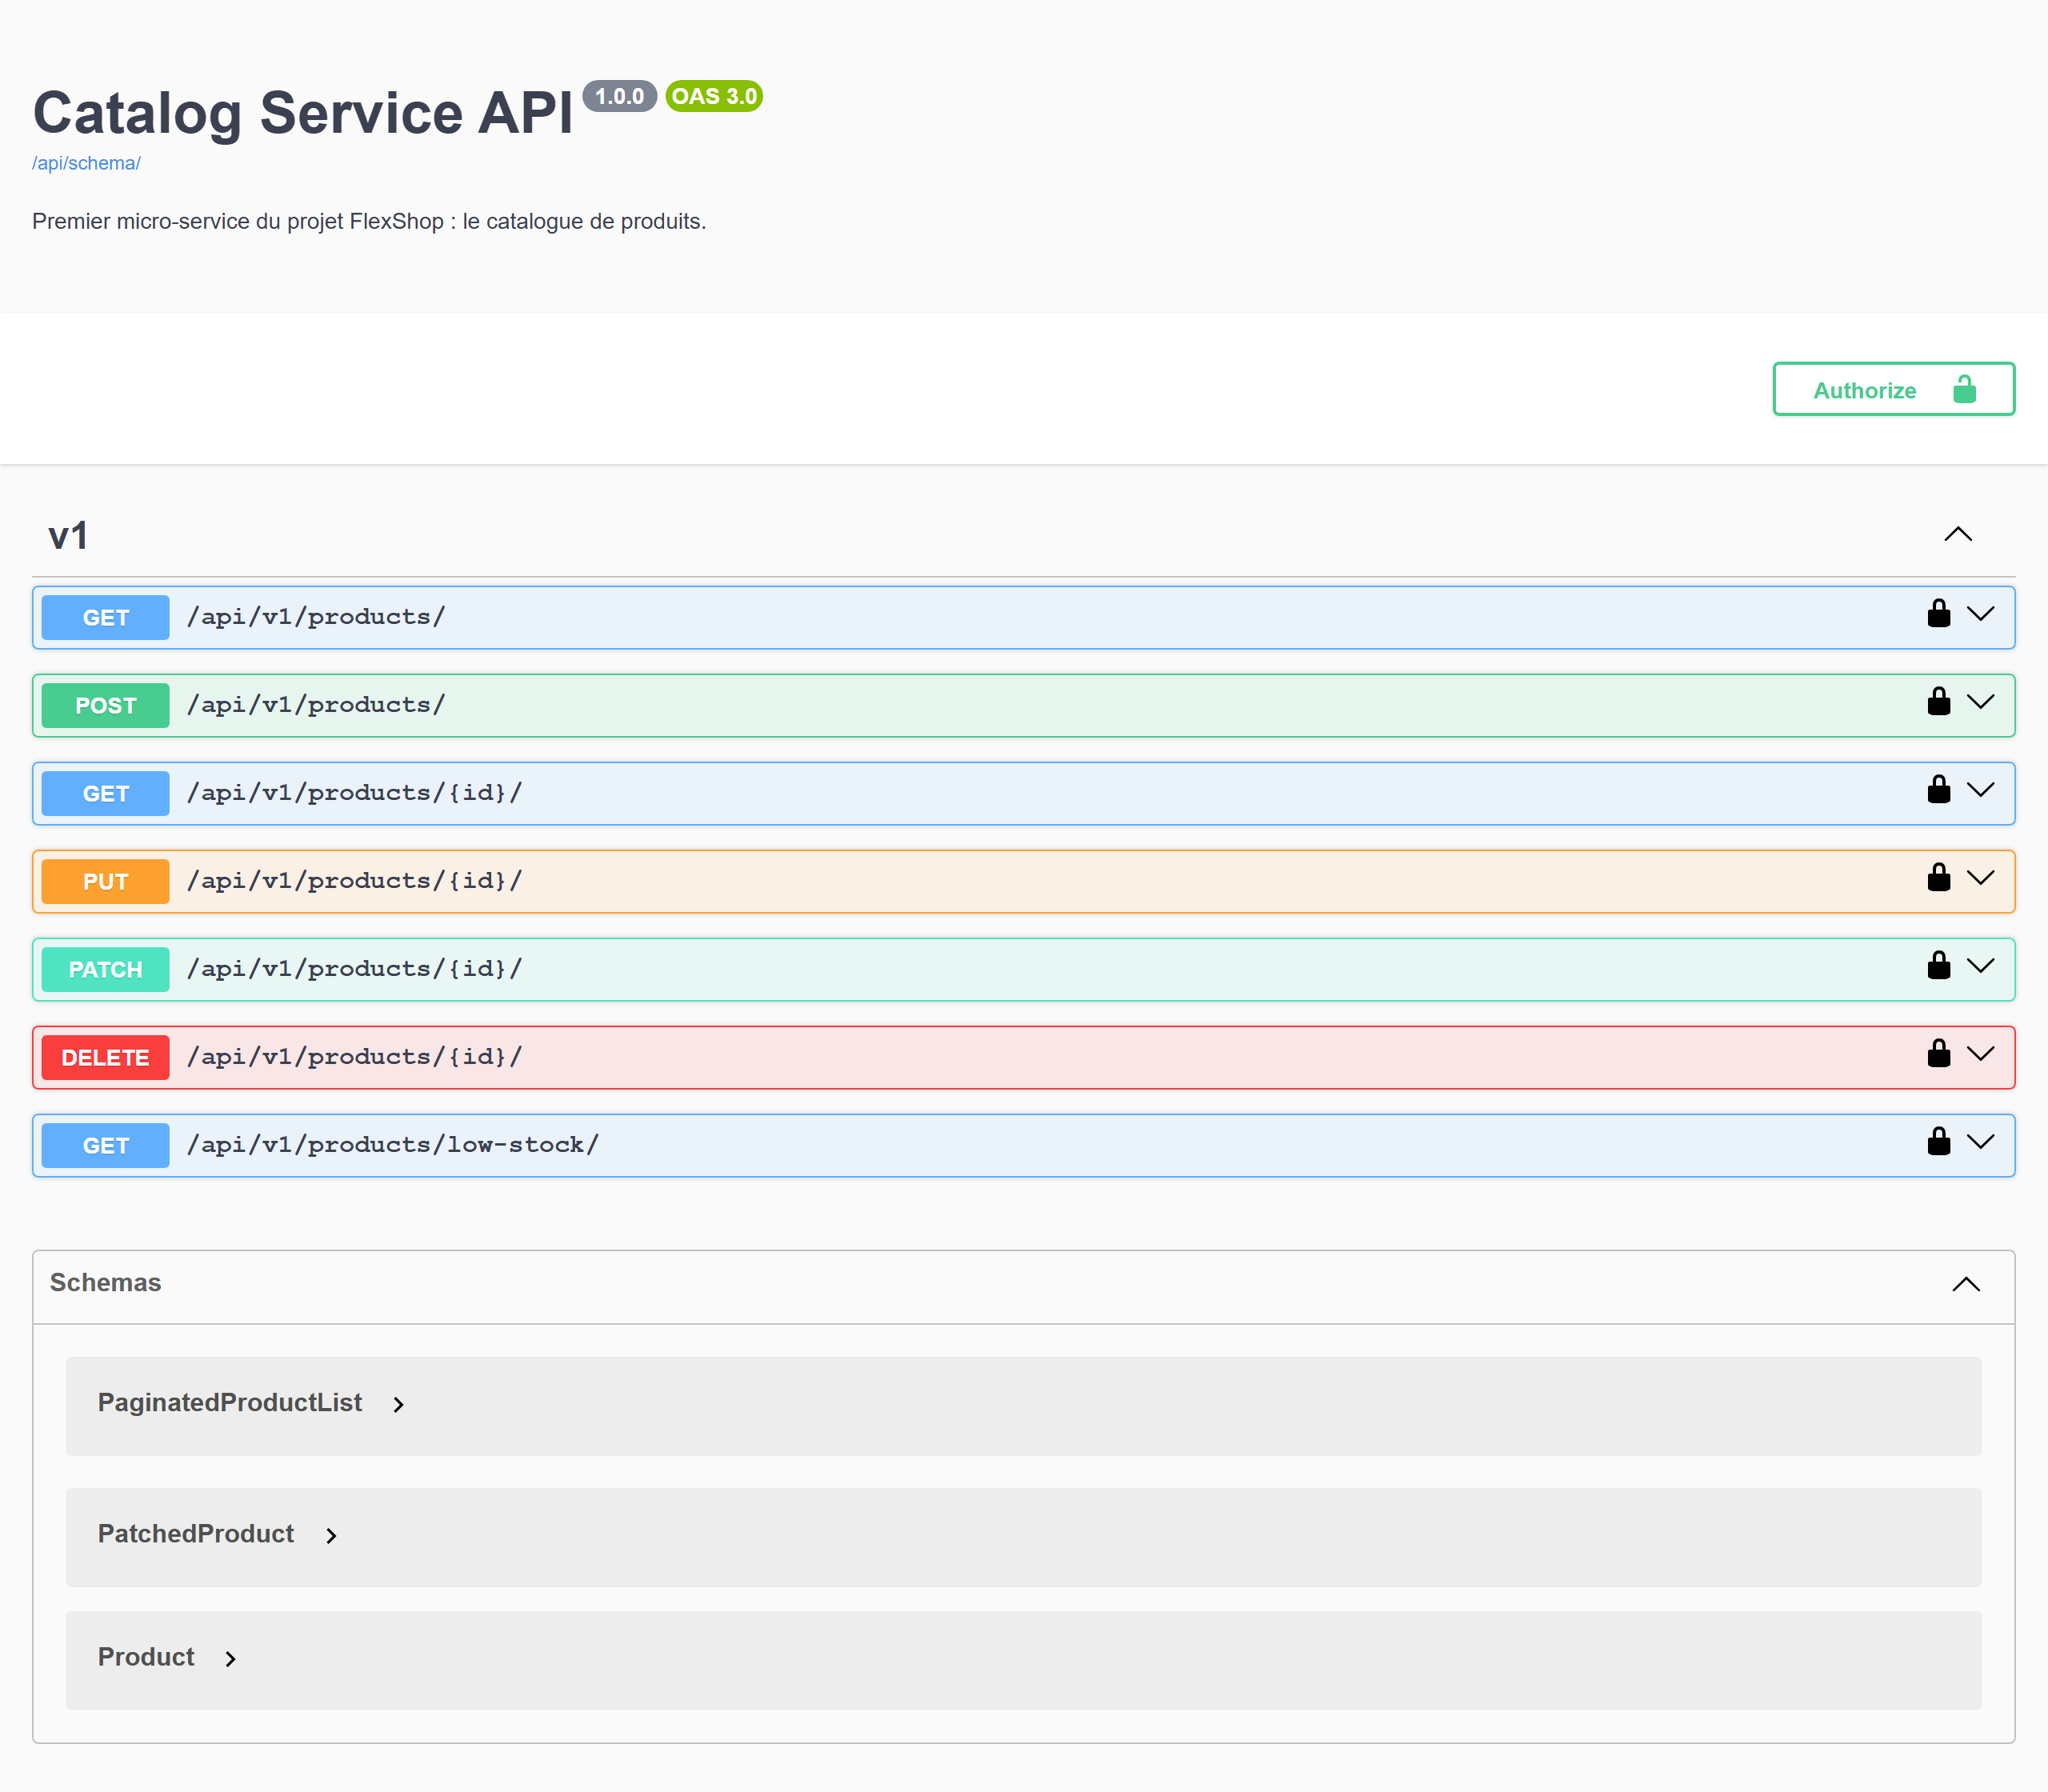
\includegraphics[width=\textwidth]{swagger-ui.png}
  \caption{Swagger UI du service Catalogue (\texttt{http://localhost:8000/api/docs/}).}
  \label{fig:swagger}
\end{figure}

\subsection{Collection Postman (\texttt{CatalogService.postman\_collection.json})}

La collection \textbf{Catalog Service -- FlexShop} fournie avec le projet regroupe \textbf{10 requêtes} prêtes à l'emploi, couvrant tout le CRUD ainsi que le filtrage, la recherche, le tri et le bonus :

\begin{itemize}
  \item \texttt{GET} Lister les produits \textperiodcentered{} \texttt{GET} Détail produit \textperiodcentered{} \texttt{POST} Créer un produit
  \item \texttt{PATCH} Modifier partiellement \textperiodcentered{} \texttt{PUT} Remplacer \textperiodcentered{} \texttt{DELETE} Supprimer
  \item \texttt{GET} Recherche (\texttt{?search=casque}) \textperiodcentered{} \texttt{GET} Tri par prix décroissant (\texttt{?ordering=-price}) \textperiodcentered{} \texttt{GET} Filtre par catégorie (\texttt{?category=})
  \item \texttt{GET} Bonus -- stock faible (\texttt{/products/low-stock/})
\end{itemize}

\subsection{Extraits de code marquants}

\textbf{Le modèle \texttt{Product}} — le prix en \texttt{DecimalField} avec validateur (jamais \texttt{FloatField}) :

\begin{lstlisting}[language=Python]
class Product(models.Model):
    name        = models.CharField(max_length=200)
    description = models.TextField(blank=True, default='')
    price       = models.DecimalField(
        max_digits=10, decimal_places=2,
        validators=[MinValueValidator(0)],   # prix >= 0
    )
    stock       = models.PositiveIntegerField(default=0)
    category    = models.CharField(max_length=50, blank=True, default='')
    created_at  = models.DateTimeField(auto_now_add=True)
    updated_at  = models.DateTimeField(auto_now=True)
\end{lstlisting}

\textbf{Le \texttt{ViewSet}} — tout le CRUD + les 3 backends de filtre + l'endpoint bonus \texttt{@action} :

\begin{lstlisting}[language=Python]
class ProductViewSet(viewsets.ModelViewSet):
    queryset = Product.objects.all()
    serializer_class = ProductSerializer
    filter_backends = [DjangoFilterBackend, SearchFilter, OrderingFilter]
    filterset_fields = ['category']               # ?category=electronics
    search_fields    = ['name', 'description']    # ?search=casque
    ordering_fields  = ['price', 'created_at', 'stock']

    @action(detail=False, methods=['get'], url_path='low-stock')
    def low_stock(self, request):                 # bonus : stock < 5
        produits = self.get_queryset().filter(stock__lt=5)
        ...
\end{lstlisting}

\subsection{Tests unitaires (6 tests, tous au vert)}

Les tests couvrent : liste, création (201), 404, prix négatif rejeté (400), suppression (204) et recherche.

\begin{lstlisting}
$ python manage.py test products
Ran 6 tests in 0.071s

OK
\end{lstlisting}

\subsection{Choix techniques notables}

\begin{itemize}
  \item Montants en \texttt{DecimalField} (\texttt{max\_digits=10, decimal\_places=2}) et \textbf{jamais} \texttt{FloatField} (les arrondis binaires sont une faute éliminatoire). On stocke \texttt{89.90} directement, ce qui reste lisible dans le JSON. L'alternative fintech (Stripe/PayPal) serait un \texttt{IntegerField} en centimes (\texttt{8990}).
  \item Validation métier dans le serializer avec \texttt{validate\_price} (prix $\geq$ 0) et \texttt{validate\_name} (nom non vide). DRF renvoie alors un \texttt{400} précis sur le champ fautif.
  \item \texttt{ModelViewSet} + \texttt{DefaultRouter} donnent tout le CRUD (list, retrieve, create, update, partial\_update, destroy) en moins de 20 lignes utiles. C'est la puissance de DRF.
  \item Filtrage, recherche et tri activés via les trois backends : \texttt{DjangoFilterBackend} (\texttt{?category=}), \texttt{SearchFilter} (\texttt{?search=} sur name + description), \texttt{OrderingFilter} (\texttt{?ordering=-price}).
  \item Pagination par défaut avec \texttt{PageNumberPagination} et \texttt{PAGE\_SIZE = 10}, soit une réponse \texttt{\{ count, next, previous, results \}}.
  \item Versioning par URI (\texttt{/api/v1/products/}).
  \item Documentation OpenAPI 3 générée automatiquement par drf-spectacular (Swagger UI sur \texttt{/api/docs/}, schéma exporté dans \texttt{openapi-schema.yml}), avec une collection Postman fournie.
  \item En bonus, un endpoint custom \texttt{@action} \texttt{GET /api/v1/products/low-stock/} liste les produits dont le stock est $<$ 5 (réapprovisionnement à prévoir).
\end{itemize}

\subsection{Difficultés rencontrées et solutions}

\begin{tabularx}{\textwidth}{@{}p{5.8cm}Y@{}}
\toprule
\textbf{Difficulté} & \textbf{Solution} \\
\midrule
\texttt{ModuleNotFoundError} au lancement. & venv non activé. Réactiver (\texttt{venv\textbackslash Scripts\textbackslash activate} sous Windows) et vérifier le prompt \texttt{(venv)}. \\[4pt]
Erreur «~App 'products' isn't installed~». & Ajouter \texttt{'products'} dans \texttt{INSTALLED\_APPS}. \\[4pt]
Changements du modèle non pris en compte. & Après toute modif de \texttt{models.py}, lancer \texttt{makemigrations} puis \texttt{migrate}. \\[4pt]
POST renvoyait \texttt{415 Unsupported Media Type}. & Dans Postman, régler Body $\rightarrow$ raw $\rightarrow$ JSON (et non Text). \\[4pt]
POST renvoyait \texttt{400} sans raison claire. & Lire le corps de la réponse. DRF indique précisément le champ en erreur. \\[4pt]
Risque de committer \texttt{db.sqlite3} et \texttt{venv/}. & Écrire le \texttt{.gitignore} \textbf{avant} le premier ajout (\texttt{venv/}, \texttt{\_\_pycache\_\_/}, \texttt{*.pyc}, \texttt{db.sqlite3}, \texttt{.env}). \\
\bottomrule
\end{tabularx}

\subsection{Ce qui resterait à améliorer pour aller en production}

\begin{itemize}
  \item \textbf{Base de données.} Remplacer SQLite par PostgreSQL, sortir \texttt{SECRET\_KEY} et \texttt{DEBUG} dans des variables d'environnement (\texttt{.env}) et passer \texttt{DEBUG=False}.
  \item \textbf{Sécurité.} Authentification et autorisation (JWT), permissions par rôle, CORS restreint, rate limiting.
  \item \textbf{Robustesse.} Erreurs au format RFC 7807, gestion fine des conflits (409), healthcheck (\texttt{/health}) pour l'orchestrateur.
  \item \textbf{Performance.} Pagination cursor-based pour un très grand catalogue, index sur les champs filtrés et recherchés.
  \item \textbf{Exploitation (DevOps).} Conteneurisation Docker, pipeline CI/CD (tests + lint automatiques), observabilité (logs structurés, métriques, tracing distribué).
  \item \textbf{Tests.} Étendre la couverture (PUT/PATCH, filtres, pagination, cas limites) au-delà des 6 tests actuels.
\end{itemize}

\end{document}
